\documentclass[11pt,twocolumn]{article}
\usepackage[a4paper,margin=0.60in,columnsep=0.25in]{geometry}
\usepackage{amsmath,amssymb,booktabs,graphicx,array}
\usepackage[hidelinks]{hyperref}
\usepackage{xurl}
\hypersetup{pdftitle={ARX--RBF Motion Modeling for Cyberattack Detection and Recovery Monitoring in Industrial Robots},pdfauthor={Muhammad Usman}}
\DeclareMathSizes{10}{10}{8}{6}
% Use cached class resources with a 10/11pt body and compact journal headings.
\makeatletter
\renewcommand{\normalsize}{\@setfontsize\normalsize{10}{11}\abovedisplayskip8pt plus2pt minus3pt\belowdisplayskip8pt plus2pt minus3pt\abovedisplayshortskip0pt plus3pt\belowdisplayshortskip5pt plus3pt minus3pt}
\renewcommand\section{\@startsection{section}{1}{\z@}{-2.5ex plus -1ex minus -.2ex}{1.2ex plus .2ex}{\normalfont\large\bfseries\raggedright}}
\renewcommand\subsection{\@startsection{subsection}{2}{\z@}{-2ex plus -.5ex minus -.2ex}{.8ex plus .2ex}{\normalfont\normalsize\bfseries\raggedright}}
\renewcommand\subsubsection{\@startsection{subsubsection}{3}{\z@}{-1.8ex plus -.5ex minus -.2ex}{.6ex plus .2ex}{\normalfont\normalsize\itshape\raggedright}}
\makeatother
\setlength{\emergencystretch}{2em}
\raggedbottom
\setlength{\textfloatsep}{11pt plus 2pt minus 2pt}
\setlength{\dbltextfloatsep}{12pt plus 2pt minus 2pt}
\setlength{\floatsep}{10pt plus 2pt minus 2pt}
\renewcommand{\topfraction}{0.9}
\renewcommand{\dbltopfraction}{0.9}
\setcounter{dbltopnumber}{4}\setcounter{totalnumber}{6}
\renewcommand{\textfraction}{0.07}
\renewcommand{\floatpagefraction}{0.8}
\renewcommand{\dblfloatpagefraction}{0.8}
\newtheorem{proposition}{Proposition}
\newenvironment{proof}{\par\noindent\textit{Proof.}\ }{\hfill\textit{Q.E.D.}\par}
\title{ARX--RBF Motion Modeling for Cyberattack Detection and Recovery Monitoring in Industrial Robots}
\author{Muhammad Usman\\[3pt]\normalsize COMSATS University Islamabad, Sahiwal Campus, Pakistan}
\date{}
\begin{document}
\makeatletter
\twocolumn[\begin{@twocolumnfalse}
\vspace{-12pt}\maketitle\vspace{-12pt}
\begin{abstract}
A robot can continue to deviate from its intended motion after an unauthorized command ends. A detector that follows recent measurements may lose evidence of that deviation, whereas an inaccurate protected reference may keep an alarm active after recovery. We study this trade-off using a command-driven motion reference, a learned residual correction and explicit alarm-clearance rules. Clean commissioning data select the reference and correction; normal calibration fixes thresholds before attack evaluation. Seventeen controls and ablations are evaluated on 189 synthetic episodes with model mismatch, legitimate command changes and unauthorized motion. The proposed nonlinear correction reduces benign alarm points from 7,156 to 7,012 relative to the uncorrected dual-window reference, but fails the declared improvement criterion: the reduction is 2.01\%, one plant worsens, and pre-return gaps increase. The short window changes no alarm decisions. A following predictor achieves higher schedule F1 but loses evidence before physical return much more often. Separate commissioning, uncertainty and common-input inertial-sensing studies explain limits of reference accuracy and recovery evidence. The results support distinguishing attack detection from physical return and reporting their costs together; they do not establish a novel detector or superiority over published robotic systems.
\end{abstract}
\noindent\textbf{Keywords:} digital twins; industrial robots; anomaly detection; recovery monitoring; system identification; model mismatch.
\vspace{12pt}
\end{@twocolumnfalse}]
\makeatother
\section{Introduction}

An industrial robot does not necessarily return to its intended trajectory when an unauthorized command stops. Its position and velocity reflect the earlier disturbance, the controller's response and the plant dynamics. An alarm that clears as soon as prediction error falls can therefore disappear while the robot is still displaced. The opposite error is also possible: the robot returns, but an inaccurate reference keeps the alarm active. These two failures concern the meaning of the reference as much as the accuracy of the detector.

Digital twins provide a useful setting for studying this problem because they connect observations with a representation of the physical process. Recent surveys cover their roles in security monitoring and infrastructure lifecycle security~\cite{securitysurvey,lifecycle}. Those roles require more than a low forecasting error. A reference must represent the behavior relevant to the decision. For an attack alarm, that may be the motion the robot would have followed under approved commands, rather than the next motion most consistent with recent measurements.

Robotic anomaly detectors such as CASPER and its edge-computing successor learn regularities in external motion sensing~\cite{casper,edge}. Hybrid robot twins also combine mechanical, control and learned components~\cite{hybrid}. These approaches motivate prediction-based monitoring, but they do not make all prediction residuals interchangeable. An observation-following predictor may become accurate during a sustained unauthorized trajectory. A command-driven reference can retain the discrepancy, provided its clean initialization and approved-command history remain trustworthy. Its accuracy under legitimate changes then becomes central to false alarms and clearance.

We ask: \emph{when does a command-driven motion reference provide useful evidence for clearing an alarm under model mismatch?} The study assumes a protected copy of approved commands and noisy but honest joint measurements. It tests an explicit candidate: a stable autoregressive reference with a frozen radial-basis correction, followed by short- and long-window return checks. The correction is fitted on clean commissioning data; it cannot learn from an attack during monitoring. This choice makes the information boundary inspectable, but does not establish either algorithmic novelty or physical safety.

The investigation proceeds through five linked validation studies. An initial recovery experiment motivates a clean-data identification study; a separate inertial-sensing study checks predictor training under common inputs; a residual experiment isolates uncertainty in windowed return evidence; and a frozen candidate audit measures detection, false alarms, recovery and component effects together. Later designs use earlier outcomes as development evidence. They do not retroactively become independent confirmations of the earlier hypothesis. This distinction follows the broader need to separate model selection from security evaluation~\cite{arp}.

The comparison separates three questions. Can clean commissioning improve reference accuracy across the declared mismatch conditions? Does the improved reference reduce benign alarms while retaining evidence through sustained corruption? Which component, if any, explains that benefit? These questions require different measurements: normal prediction error, the complete alarm trajectory, and matched component removals. A single F1 value cannot answer all three.

The contributions supported by the completed work are threefold. First, we specify and test a command-driven reference and alarm-state model with an explicit separation between observed residuals and evaluator-only physical return. Second, matched controls and ablations show that protected reference evolution, nonlinear correction and alarm persistence have different effects: the simpler reference retains the main benefit, while the proposed correction fails its improvement criterion. Third, commissioning and uncertainty diagnostics explain why better prediction alone may not yield usable return evidence. These are empirical and methodological findings. The present evidence does not validate a new state-of-the-art detector.


The remainder of the paper separates these decisions. Section~\ref{sec:literature} positions the study in prior work. Sections~\ref{sec:methods}--\ref{sec:comparators} define the model, experiments, metrics and comparison methods. Section~\ref{sec:results} reports the complete outcomes; Sections~\ref{sec:discussion} and~\ref{sec:conclusion} interpret their scope. The appendices retain uncertainty derivations, earlier results and source identities within this article.

\section{Literature Review}\label{sec:literature}

\subsection{Robot monitoring and reference identification}
CASPER couples external inertial sensing with context-aware industrial-arm anomaly detection~\cite{casper}. The subsequent edge study develops real-time processing for related robotic monitoring~\cite{edge}. Their sensing modality differs from the joint positions, velocities and protected commands used here. We therefore examine independently implemented CNN predictors on a common nominal inertial recording in a separate track. An error measured in that track cannot be interpreted as attack-detection superiority over either complete published system.

Ayankoso et al. combine robot mechanics, drives, control and learned uncertainty accommodation in a hybrid condition-monitoring twin~\cite{hybrid}. Data-driven robot calibration is itself a broad research area~\cite{calibration}; adding a learned correction to a nominal reference is not sufficient evidence of novelty. Classens et al. address structured mechanical-system identification using instrumental variables and block-coordinate descent~\cite{identification}. Our finite autoregressive search uses ordinary least-squares regularization and tests an application-specific recovery requirement, rather than extending that identification theory.

The voraus-AD study provides real robot executions and MVT-Flow, a normalizing-flow anomaly detector~\cite{voraus}. It is a relevant public comparator for an independent real-robot track because both data and author code can be inspected. Its published full-execution likelihood is an offline episode score. Comparing it directly with an online alarm-clearance delay would change the task. FactoryNet extends public industrial data coverage and exposes setpoints, effort, feedback and context in a common schema~\cite{factory}. Its latest manuscript is a preprint, and its releases combine new acquisitions with repackaged sources. Independence must be assessed by acquisition, not by dataset name.

\subsection{Forecasting, uncertainty and runtime decisions}
ModernTCN examines convolutional time-series modeling~\cite{moderntcn}, iTransformer attends across variates for forecasting~\cite{itransformer}, and TimeMixer uses decomposable multiscale mixing~\cite{timemixer}. These recent architectures offer useful forecasting alternatives, but architecture size alone does not solve the reference problem. A more accurate predictor of corrupted motion can be less useful for retaining attack evidence. None of these three systems is claimed as an executed comparator in this study.

Interval-observer fault detection already treats model uncertainty and observer design explicitly~\cite{interval}. FAIL-Detect calibrates uncertainty-aware runtime failure monitors from successful robot rollouts~\cite{fail}. We include a constant episode-band control inspired by that calibration principle in the earlier experiment, without claiming to reproduce its policy-specific signal construction or full method. Howard et al. develop time-uniform confidence sequences~\cite{howard}; our Gaussian window diagnostic uses simpler tail bounds and error spending under stated assumptions.

Kaisar et al. describe a robotic-vehicle cybersecurity architecture involving a kinematic twin, supervisory handover and consistency-gated recovery~\cite{kaisar}. This is close conceptual prior art. The available abstract supports that overlap, but the full algorithm was inaccessible during our audit, leaving an equation-level comparison unresolved. RESCUE uses counterfactual interventions to evaluate the usefulness of runtime alarms~\cite{rescue}. Our counterfactual serves a narrower purpose: measuring when a simulated plant returns to the trajectory it would have followed without command corruption.

Evaluation also matters. TSB-AD examines the reliability of time-series anomaly-detection comparisons~\cite{tsbad}, while VUS studies accuracy measures for temporal anomalies~\cite{vus}. We retain unadjusted point metrics and separately report event detection and recovery. We do not adopt point adjustment or optimize a threshold on test attacks.

\subsection{Limitations and unresolved comparison requirements}
The literature supports the individual ingredients of prediction, correction, uncertainty calibration and persistent alarm state. It does not justify treating their combination here as automatically new. The principal comparison gaps are specific: different sensing modalities for CASPER, a full-execution objective for MVT-Flow, unresolved implementation correspondence for some published systems, and missing physical-return labels in public fault data. These are limits on what our experiment can establish, not evidence that the cited systems are generally defective. A claim of superiority requires a compatible implementation and matched information access.


\section{Methods}\label{sec:methods}
\subsection{State, information and threat model}
Let $x_t=(q_1,q_2,\dot q_1,\dot q_2)$ be the physical state and $x_t^0$ the state of the same plant under the complete approved command history without corruption. The monitor observes $y_t=x_t+n_t$ and approved position/velocity commands $u_t$. Its maintained state comprises predicted-state and command histories, residual buffers, an alarm bit and a return counter. The evaluator alone receives $x_t$, $x_t^0$ and the corruption schedule. Figure~\ref{fig:model} shows this information boundary.

The attacker changes commands delivered downstream of a protected command copy. Clean commissioning data, the first 100 initialization observations and that copy are trusted. Measurements contain noise, but adversarial sensor forgery is outside this experiment. Once initialized, the protected reference consumes no new measured state. This prevents corrupted motion from changing its predicted history or fitted parameters. It is conditional on the protected inputs, and does not address compromise of both commands and telemetry.

The reference estimates the response to approved commands, initialized from the clean prefix and synchronized through command timing. It is an empirical motion reference, without online parameter adaptation or validated industrial physical fidelity.

\begin{figure*}[t]
\centering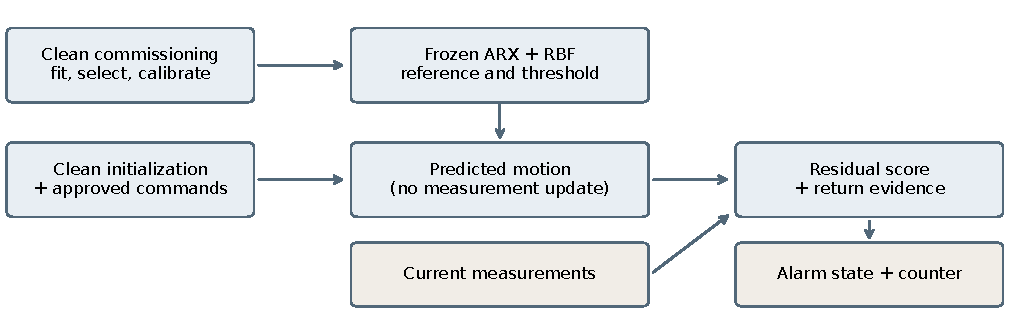
\includegraphics[width=0.82\textwidth]{figures/model.pdf}
\caption{Tested reference and alarm model. Clean data determine the frozen recurrence, correction and threshold. Approved commands drive the reference after initialization. Measurements determine residuals and alarm state, without updating the reference. Counterfactual physical return is restricted to evaluation.}\label{fig:model}
\end{figure*}

\subsection{Stable command-driven reference}
The base is a clean-data autoregressive model with exogenous inputs (ARX). In its fitted coordinates,
\begin{align}
 b_t&=a+\sum_{k=1}^{p}A_k b_{t-k}+\sum_{k=1}^{p}B_k u_{t-k},\label{eq:base}\\
 r_t^0&=\mu+s\odot b_t .
\end{align}
Commands retain their recorded physical coordinates. Training supplies state location $\mu$ and positive scales $s$; constant or nonfinite state channels are rejected. After initialization, Equation~\ref{eq:base} uses predicted states in its own history. The plant-specific orders are 8, 16 and 32 for Q1--Q3, and each selected companion matrix has spectral radius below one. Stability concerns this fitted linear recurrence; it does not establish bounded physical error under arbitrary commands or guarantee transfer to a different robot.

The following control instead uses measured history to predict the next observation. This changes the reference target while retaining the available channels.

\subsection{Training-only residual correction}
A correction estimates systematic normal residuals without feeding them back into the ARX recurrence. Its feature vector is
\begin{align}
 f_t&=[r_t^0,u_{t-1},u_{t-4},u_{t-16},u_{t-32}],\\
 z_t&=(f_t-\mu_f)/s_f,\label{eq:features}
\end{align}
with 20 dimensions. The feature means and scales use training observations only; a feature scale at or below $10^{-12}$ is replaced by one. This is distinct from rejecting a constant physical-state scale. Farthest-point selection in standardized training space deterministically chooses $K$ centers $c_i$, starting from the observation closest to the origin. The bandwidth $h$ equals a selected multiplier times the median positive center distance.

The radial basis functions (RBFs) and corrected output are
\begin{align}
 \phi_i(z)&=\exp\{-\|z-c_i\|_2^2/(2h^2)\},\\
 r_t&=r_t^0+s\odot W^T[\phi_1(z_t),\ldots,\phi_K(z_t),1]^T.\label{eq:rbf}
\end{align}
The four-output coefficient matrix minimizes
\begin{equation}
 N^{-1}\|\Phi W-E\|_F^2+\lambda\|W_{1:K,:}\|_F^2,\label{eq:fit}
\end{equation}
where $E$ contains standardized clean residuals. The intercept is unpenalized, and nonfinite fits are rejected. A linear correction uses the same 20 standardized features and objective, providing a direct nonlinearity control. RBF heads contain $4(K+1)$ coefficients: 132 for 32 centers and 260 for 64 centers. These counts exclude stored centers, feature statistics and the base ARX. The linear head contains 84 coefficients.

Bounded activations and fixed weights bound correction magnitude, not physical prediction error. Weights, centers, scales and thresholds remain frozen during evaluation.

\subsection{Entry score and alarm-clearance state}
Define $e_t=(y_t-r_t)/s$ and $a_t=\max_j|e_{t,j}|$. Strict exceedance $a_t>\tau$ raises an alarm and resets its return counter. At other eligible points, the candidate checks
\begin{equation}
 g_t=\mathrm I\!\left\{\|\bar e_t(5)\|_\infty\le0.1\ \land\
 \|\bar e_t(41)\|_\infty\le0.1\right\},\label{eq:gate}
\end{equation}
where $\bar e_t(m)=m^{-1}\sum_{k=0}^{m-1}e_{t-k}$. Ten consecutive qualifying points clear an active alarm; a new entry exceedance has priority. The windows contain 0.10 and 0.82 seconds of samples at 50 Hz, and the dwell contains 0.20 seconds. Only complete windows after the initialization prefix are eligible. Signed means can cancel oscillatory deviations, so the gate measures agreement with the reference rather than certifying physical return.

Invalid history resets the evidence streak and cannot clear an active alarm; the implemented known-state mask then remains false. The final campaign admits complete finite episodes, so missing-data behavior is software-tested only. Algorithm~\ref{alg:replay} specifies the causal order.

\begin{table*}[t]\centering
\caption{Algorithm 1: normal-only fitting, selection and freezing.}
\label{alg:fit}
\begin{tabular}{>{\raggedright\arraybackslash}p{0.055\textwidth}>{\raggedright\arraybackslash}p{0.88\textwidth}}\toprule
Input & Separate clean training, development and calibration episodes; declared candidate grid and tie-break rule.\\\midrule
1 & Fit training-only state statistics and candidate ARX references; reject invalid or unstable candidates. Preserve each candidate outcome.\\
2 & Generate free-running training predictions from clean initial histories. Construct the 20-dimensional features and fit their statistics and centers on training only.\\
3 & Solve the ridge objectives. Evaluate each frozen candidate on the same normal-development episodes, keeping episode boundaries intact.\\
4 & Within the linear and RBF roles separately, select by worst-episode residual $q_{.99}$, then mean RMSE, coefficient count and identifier. Preserve the chosen artifact without refitting on development.\\
5 & Score the separate normal-calibration population. Set the fixed entry threshold to ascending rank 5,445 of 5,500 scores.\\
6 & Seal models, transforms, thresholds, methods, seeds, inputs, code, budgets and criteria before generating the new evaluation conditions.\\\bottomrule
\end{tabular}
\end{table*}

\begin{table}[t]\centering
\caption{Algorithm 2: prospective monitoring of one episode.}\label{alg:replay}
\begin{tabular}{>{\raggedright\arraybackslash}p{0.12\columnwidth}>{\raggedright\arraybackslash}p{0.76\columnwidth}}\toprule
Input & Frozen model and threshold; clean 100-point prefix; approved commands and current measurements.\\\midrule
1 & Initialize predicted history from the prefix; set alarm and evidence counter to zero.\\
2 & Predict $b_t$ from earlier predicted states and commands; compute $r_t$ using the frozen correction.\\
3 & Read $y_t$, calculate $e_t,a_t$, and update the complete residual windows. No label or future measurement is read.\\
4 & If history is invalid, reset the streak and retain alarm state. Otherwise, an entry exceedance raises alarm and resets the streak.\\
5 & If alarm is active without an exceedance, increment the streak when $g_t=1$, otherwise reset it. Clear after the declared dwell.\\
6 & Save score, validity and alarm at index $t$. Advance predicted history, leaving fitted parameters fixed. Continue across attack boundaries.\\\bottomrule
\end{tabular}
\end{table}

\subsection{Physical return and uncertainty}
The evaluator measures $d_t=\max_j|x_{t,j}-x_{t,j}^0|/s_j$. Reference/noise bounds $b_t,\eta_t$ would give $d_t\le a_t+b_t+\eta_t$. Sufficient return requires $a_t+b_t+\eta_t\le\delta$, which is infeasible when the allowance exceeds the tolerance. Empirical maxima under Gaussian noise are not deterministic bounds. Appendix~\ref{app:uncertainty} develops this limitation and the window diagnostic.

\section{Experiments}\label{sec:experiments}
\subsection{Datasets and experimental populations}
The study separates simulated attack/recovery evaluation, real-data normal prediction and admission of future public evidence (Table~\ref{tab:data}). They answer different questions and are not pooled into one performance ranking. Five linked studies document the development sequence (Table~\ref{tab:studies}). Later choices use earlier outcomes as development; the earlier studies do not become independent confirmations of those choices.

\begin{table*}[t]\centering
\caption{Data and information boundaries. Counts identify the populations actually used or admitted. New public-data receipt is not an additional experiment.}\label{tab:data}
\begin{tabular}{>{\raggedright\arraybackslash}p{0.18\textwidth}>{\raggedright\arraybackslash}p{0.23\textwidth}>{\raggedright\arraybackslash}p{0.26\textwidth}>{\raggedright\arraybackslash}p{0.23\textwidth}}\toprule
Source & Population & Permitted model information & Status and interpretation\\\midrule
Two-joint simulation, E5 & 3 training, 9 development and 5 calibration episodes per plant; 81 fresh normal and 189 audit episodes & Noisy joint position/velocity and protected approved commands; clean initialization & Synthetic, with evaluator-only command intervals and same-plant physical-return truth.\\
CASPER provider-v2 nominal IMU, E3 & 8,192 common training and 2,048 development targets; nine channels & Past causally filtered accelerometer, gyroscope and magnetometer observations & Real nominal prediction; no attack evaluation, unresolved paper-release and clock correspondence.\\
voraus-AD original 100 Hz release & 2,122 executions; original split 948 training / 1,174 test & No process signals admitted to modeling yet & Metadata verified only; normal/fault labels, no established cyber or physical-return labels.\\
FactoryNet & Author-reported mixed real/synthetic corpus & No observations downloaded & Partially admitted source; imported sources are not new independent acquisitions.\\\bottomrule
\end{tabular}
\end{table*}

\subsubsection{Physical simulator and command construction}
The plant is a horizontal two-joint point-mass arm:
\begin{equation}
 M(q)\ddot q+C(q,\dot q)+B\dot q=\tau.\label{eq:plant}
\end{equation}
For $a=m_2l_1l_2$ and $d=m_2l_2^2$, its inertia entries are $M_{11}=(m_1+m_2)l_1^2+d+2a\cos q_2$, $M_{12}=M_{21}=d+a\cos q_2$, and $M_{22}=d$. The Coriolis vector is $a\sin q_2[-2\dot q_1\dot q_2-\dot q_2^2,\dot q_1^2]^T$. A proportional--derivative controller requests
\begin{equation}
 \tau^*=\operatorname{clip}\{K_p(q^c-q)+K_d(\dot q^c-\dot q),-20,20\},
\end{equation}
with diagonal gains $(18,12)$ and $(4,3)$. With actuator lag, $\dot\tau=(\tau^*-\tau)/T_a$. Nominal masses are $(1,0.8)$ kg, lengths $(0.5,0.4)$ m and damping $(0.08,0.06)$; Table~\ref{tab:plants} defines the actual plants. Position and velocity noise are independent zero-mean Gaussian with standard deviations 0.0005 rad and 0.002 rad/s before the plant multiplier.

\begin{table*}[t]\centering
\caption{Fixed simulated plants. Mass and damping factors multiply the nominal values; noise multiplies both sensor standard deviations.}\label{tab:plants}
\begin{tabular}{lcccrr}\toprule
Plant & Mass factors & Damping factors & Lengths (m) & Lag (s) & Noise\\\midrule
Q1 & (1.10,0.86) & (0.80,1.20) & (0.48,0.42) & 0 & 1.0\\
Q2 & (0.88,1.15) & (1.30,0.85) & (0.53,0.37) & 0.03 & 1.0\\
Q3 & (1.16,1.06) & (0.90,1.40) & (0.46,0.43) & 0.06 & 1.5\\\bottomrule
\end{tabular}
\end{table*}

Sampling is 50 Hz with eight fourth-order Runge--Kutta substeps per sample. A separate short integration check supports numerical consistency, not fidelity to an industrial robot. Gravity, contact, flexibility and thermal effects are absent. Approved positions are
\begin{align}
 q_1^c&=a_1\sin\theta+0.025\sin(2.3\theta),\\
 q_2^c&=a_2\sin(\theta+\phi)+0.018\sin(1.7\theta),
\end{align}
with analytic velocities under the causal time warp. The final tasks are N14: $\theta=0.49t$, amplitudes $(0.28,0.37)$, phase 0.93; O14: $\theta=0.43t+0.008t^2$, amplitudes $(0.33,0.31)$, phase 0.72; and P14: $\theta=0.94t+0.18\sin(0.31t)$, amplitudes $(0.35,0.38)$, phase 1.14.

The final audit crosses these three tasks, three existing plants, seeds 17, 42 and 2026, and seven conditions: ordinary operation, authorized offset, authorized slowdown, brief unauthorized offset, persistent offset, hold and slowdown. There are 81 wholly benign and 108 attack episodes. Each contains 1,200 samples, including the clean 100-point initialization. Corruption begins at index 347 and ends before 653, except the eight-point brief offset. Offset magnitude is 0.11 rad on joint 1; slowdown rate is 0.72. Authorized changes update the approved command, while attacks change only the delivered command. Truth and schedule remain outside the inference interface.

\subsubsection{Real nominal recording and independent sources}
The separate IMU study uses the provider-v2 nominal \texttt{IMU\_10Hz.csv}, with accelerometer, gyroscope and magnetometer axes. It differs from the original CASPER-v3 archive. Exact correspondence to the published runs, timestamp units and acquisition-versus-arrival timing remain unresolved. We report sample-based prediction errors, not physical-time attack delays inferred from the filename.

voraus-AD metadata and original splits were verified, but its process signals remain unopened~\cite{voraus}. FactoryNet remains source-audited only~\cite{factory}. Appendix~\ref{app:provenance} records hashes, permissions, source overlap and code-admission issues; neither source contributes measured model results here.

\subsection{Preprocessing, chronology and calibration}
\subsubsection{Synthetic commissioning and held-out conditions}
Three clean commissioning episodes per plant fit the base and corrections. Their rates are 0.35, 0.7 and 1.1, with amplitudes $(0.22+0.04i,0.34-0.025i)$ and phase $0.5+0.3i$ for $i=0,1,2$, covering unchanged, authorized-offset and authorized-slowdown motion. The earlier normal episode bank uses rate $0.32+0.047i$, amplitudes $(0.23+0.012(i\bmod7),0.29+0.013(i\bmod9))$ and phase $0.4+0.06(i\bmod11)$. Indices 0--8 select configurations and 9--13 calibrate. Five remaining archived checks are not new independent data.

Transforms, centers and regression coefficients use training only. Each episode retains its own initialization and history; windows never cross episode or split boundaries. After selection, each reference has 5,500 eligible calibration scores. The ascending score at rank $\lceil0.99(5500)\rceil=5445$ fixes its threshold. Strict exceedance handles ties. Calibration cannot choose models, seeds or a better percentile. Equal point-score quantiles do not equalize a stateful rule's alarm occupancy or guarantee future 1\% false alarms.

The candidate check uses 81 new normal combinations based on tasks K13, L13 and M13. The attack audit freezes the fits, thresholds and 17-method roster before generating N14, O14 and P14. The tasks are new; the simulator and plants are reused. All resulting conditions are now exposed.

\subsubsection{Chronological IMU partitions}
Zero-indexed training rows $[219,9185)$ precede development rows $[9185,12007)$. Splitting occurs before the trailing width-20 median filter, training scaling and history creation. Each partition loses 19 filter warmup observations. Timestamps must increase strictly, with no gap exceeding five times the training median increment. Constant or nonfinite training channels are rejected.

All predictors share 8,192 training and 2,048 development targets after 755 history observations. Development targets are raw rows 9959--12006 inclusive. A later 755-residual aggregation has 1,294 aligned endpoints. The compact CNN uses only its 45-point history, but receives the same eligible target rows. These data were used for checkpoint selection and cannot serve as independent final evaluation.

\subsection{Experimental setup and optimization procedure}
\subsubsection{Finite model search}
The earlier reference search comprises ARX orders 4, 8, 16 and 32 and finite impulse response lengths 16, 32 and 64, crossed with ridge penalties $10^{-7},10^{-5},10^{-3}$ on each plant: 63 fits. Stable ARX orders 8, 16 and 32 with ridge $10^{-7}$ are inherited by the correction study.

The correction grid has eight RBF settings per plant: $K\in\{32,64\}$, width multiplier in $\{0.5,1\}$ and ridge in $\{0.001,0.01\}$. Two linear penalties use the same feature inputs, giving 30 fits overall. Within each correction role, selection minimizes the worst episode's 99th-percentile standardized residual, then mean episode RMSE, head coefficient count and identifier. All candidates and failures remain recorded. ``Optimal parameters'' here means selected within this finite normal-development procedure, not a global optimum or a choice based on final attacks.

\subsubsection{Neural training and stopping}
The independent CASPER-style CNN has four valid one-dimensional convolutions, each with 32 filters, kernel five and ReLU. Width-three pooling follows each pair; flattening and a nine-output dense layer give 39,977 parameters for 755-point history. The Edge-style CNN has two valid convolutions with eight filters and kernel three, width-three pooling, and a nine-output dense layer: 1,369 parameters for 45-point history. Both use zero-initialized output heads, disclosed as an implementation choice.

Adamax uses learning rate $10^{-3}$ and batches of 64 in chronological order without shuffling. A normal-development improvement greater than $10^{-6}$ selects a checkpoint; patience is five epochs and the cap is 100. Seeds 17, 42 and 2026 start afresh without optimizer transfer. No transformer is trained; the references to recent forecasting architectures establish related work, not executed baselines. Per-fit CPU admission is 240 seconds, with total limits of 1,200 seconds wall and 900 seconds CPU.

\subsubsection{Execution environment and validation sequence}
Runs use macOS/arm64, Python 3.12.15 and NumPy 1.26.4; CNNs additionally use TensorFlow 2.16.2. IMU provenance records 18 logical processors, but no verified RAM specification or GPU benchmark. Inference outputs are sealed before joint label evaluation. Exact execution records and failures are retained.

\begin{table*}[t]\centering
\caption{Five completed studies and their comparison roles. They are a development sequence, not five independent robot datasets.}\label{tab:studies}
\begin{tabular}{>{\raggedright\arraybackslash}p{0.04\textwidth}>{\raggedright\arraybackslash}p{0.22\textwidth}>{\raggedright\arraybackslash}p{0.29\textwidth}>{\raggedright\arraybackslash}p{0.34\textwidth}}\toprule
ID & Question & Evidence & Declared outcome\\\midrule
E1 & Recovery under mismatch & 216 synthetic episodes; 13 rules & Uncertainty allowance reduces alarms but prevents many clears.\\
E2 & Clean reference accuracy & 63 fits; 81 fresh normal episodes & Better fitting improves allowances; overall feasibility still fails.\\
E3 & Common-input prediction & Nominal CASPER IMU prefix; nine outcomes & AR(4) has lowest development MSE; compact CNN reaches its epoch cap.\\
E4 & Window uncertainty & 36 synthetic residual traces; six rules & Required normal feasibility holds on 20/36 traces.\\
E5 & Candidate and components & 30 fits; 81 normal and 189 audit episodes & Nonlinear dual-window candidate fails its declared advantage criterion.\\\bottomrule
\end{tabular}
\end{table*}


\section{Evaluation Metrics}\label{sec:metrics}
\subsection{Prediction and point-level detection}
For $N$ eligible targets and $d$ training-standardized channels, normal prediction error is
\begin{equation}
 \operatorname{MSE}=\frac{1}{Nd}\sum_{t,j}\left(\frac{y_{t,j}-r_{t,j}}{s_j}\right)^2,
 \qquad \operatorname{RMSE}=\sqrt{\operatorname{MSE}}.
\end{equation}
Development also uses the 99th percentile of $a_t=\|e_t\|_\infty$. A low normal error is not an attack-detection result. The same training scales are retained for each model's assigned evaluation.

Point counts compare the alarm bit with the command-corruption schedule on all eligible observations, without point adjustment:
\begin{align}
 P&=\frac{TP}{TP+FP},\quad R=\frac{TP}{TP+FN},\\
 F_1&=\frac{2TP}{2TP+FP+FN}.
\end{align}
Precision is zero when there are no positive predictions. Average precision (AP) uses continuous entry scores: $\mathrm{AP}=\sum_k(R_k-R_{k-1})P_k$, grouping equal scores at common thresholds. It is undefined with no positive labels. Gate variants can therefore share AP while producing different alarm trajectories. The final audit has 207,900 eligible points and 25,002 schedule-positive points per method, with complete score coverage.

\subsection{Benign alarms, event coverage and delay}
Benign occupancy is $N_{\rm alarm}/N_{\rm benign}$ on wholly benign episodes. Starts per hour divide alarm rising edges by $N_{\rm benign}\Delta t/3600$, where $\Delta t=0.02$ seconds. The final benign population is 89,100 points, or 0.495 eligible hours. Short repeated alarms and one sustained alarm may have similar occupancy but very different start rates.

An overlap hit is any alarm during an attack interval. A fresh hit requires a rising edge within that interval. Both denominators are all 108 events; a preexisting alarm can overlap without a fresh onset. Delays measure samples from schedule onset to the first qualifying overlap or rising edge, multiplied by $\Delta t$. Misses remain explicit, with undefined delays rather than silently removed or assigned zero. There is one scheduled intervention per attack episode; these are paired simulation conditions, not independent industrial incidents.

\subsection{Physical return and clearance}
Physical return is the first start of ten consecutive post-corruption states with $d_t\le0.1$. This retrospective evaluator label uses the uncorrupted same-plant trajectory and never enters inference. Timely clearance is an inactive alarm at or within 250 samples after that return. The ratio conditions on detected events for which physical return exists; an already inactive alarm has zero clearance delay. This definition must be read alongside early clearance and misses.

The registered early-clear metric records a falling edge after first overlap but before stable physical return. Gap points count inactive observations between that hit and return, or the episode end when no return exists. A continuity break near onset can count even while instantaneous deviation is small. An explicitly post-study diagnostic separately checks true deviation at early falling edges; it does not replace the registered outcome.

\subsection{Predeclared improvement and cost}
RBF dual must preserve or improve hits, fresh hits and timely clears on each plant, while not increasing early-clear events, benign alarm points or pre-return gaps. It must also reduce pooled benign points or gaps by at least 10\% relative to base dual. These are descriptive registered requirements, not statistical noninferiority tests. Secondary metrics cannot rescue a failed primary criterion.

Wall time, worker CPU, sampled resident memory and output size measure whole recorded runs. Shared computation prevents interpreting total time divided by the number of methods as per-method latency. Stochastic seeds describe computational/noise variation within the same experimental systems; no confidence interval is presented as if they were independent robot acquisitions.


\section{Comparison Methods and Baselines}\label{sec:comparators}
\subsection{Protected references and component removals}
The final roster compares base ARX, linear correction and RBF correction under matched inputs. Point rules directly threshold $a_t$. Return rules retain alarm using a one-point residual condition, the 41-point window, or the 5/41 dual window, generally with ten-point dwell. The no-dwell variant requires one qualifying point. Base long versus base dual and RBF long versus RBF dual isolate the short window; RBF dual versus its no-dwell variant isolates persistence. Base dual versus RBF dual is the primary correction comparison. Every variant keeps its declared entry score, threshold and support.

The RBF-following ablation applies the correction trained on free-running features to measured-history predictions without refitting. It tests that disclosed assembly, not an optimally fitted following model. Table~\ref{tab:audit} retains all 17 methods.

\subsection{Ordinary prediction and accumulation controls}
Persistence predicts the last measured state. The causal rolling mean predicts from the preceding 21 observations, excluding the current target. A one-sided CUSUM uses $G_t=\max(0,G_{t-1}+a_t-k)$, with $k$ equal to the training-score mean plus its standard deviation. Its calibrated statistic has no reset on alarm in this registered implementation. Its persistence is therefore a deliberate comparator behavior, not a claim that all CUSUM schemes cannot recover. All controls use identical eligible episode support and cannot access labels or truth.

The IMU controls are training mean, persistence and AR(4), alongside the CNNs specified in Section~\ref{sec:experiments}. AR fits standardized channels with ridge $10^{-3}$ on mean normal equations, leaving its intercept unpenalized. Deterministic controls run once and neural models use all three seeds.

\subsection{Published-method correspondence}
CASPER and its successor motivate the CNN architectures, but E3 uses independent implementations, a different normal-only protocol and a provider release whose original-run correspondence is unresolved. It is not a reproduction of their complete attack detectors. Their external IMU inputs also differ from the joint telemetry and protected commands in E5. Published headline metrics are not inserted into our measured ranking.

MVT-Flow is a public author-code candidate for a separate offline real-robot study. Full-execution likelihood, symmetric temporal convolutions and unresolved released-code objective/layer correspondence prevent immediate admission as an online recovery comparator. ModernTCN, iTransformer and TimeMixer remain architectural background. No execution result is attributed to any unrun method. This separation makes the scientific gap explicit: the present controls test mechanism behavior, while a compatible full published-baseline reproduction remains unfinished.


\section{Results}\label{sec:results}
\subsection{Parameter selection and normal prediction}
The 63-fit E2 search selects ARX orders 8, 16 and 32 with ridge $10^{-7}$. Its complete normal comparison is retained in Appendix~\ref{app:earlier}. For the E5 correction, all 30 candidates produce eligible outcomes. Figure~\ref{fig:tuning} displays every development criterion, including weaker settings. Selection chooses 32 centers on all plants, width multipliers 1, 0.5 and 1, and penalties 0.01, 0.001 and 0.001 for Q1--Q3. All selected linear penalties are 0.01. These are finite normal-development choices, not parameter choices based on the attack audit.

\begin{figure*}[t]\centering
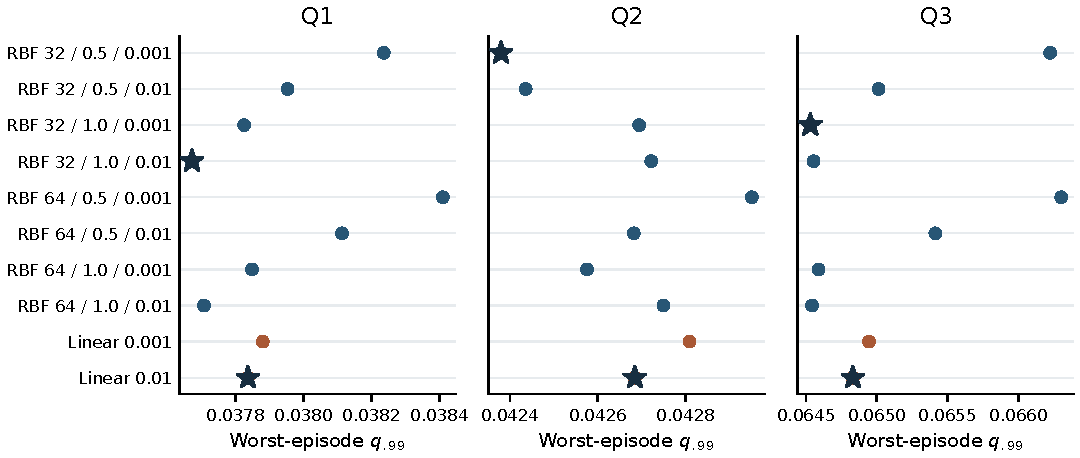
\includegraphics[width=\textwidth]{figures/tuning.pdf}
\caption{All 30 correction candidates on normal development: worst-episode 99th-percentile standardized residual (lower is better). RBF labels give centers/width multiplier/ridge; linear labels give ridge. Stars mark the selected candidate within each correction role on each plant. Horizontal scales differ across panels. These are selection outcomes, not held-out attack results.}\label{fig:tuning}
\end{figure*}

\begin{table*}[t]\centering
\caption{Selected E5 candidate and fresh-normal changes against the base reference. Positive error change is worse. Each selected RBF head has 132 coefficients, in addition to its stored centers and base model.}\label{tab:selection}
\begin{tabular}{lrrrrrrr}\toprule
Plant & ARX $p$ & Centers & Width & Ridge & $\tau$ & $\Delta$RMSE (\%) & $\Delta q_{.99}$ (\%) \\\midrule
Q1 & 8 & 32 & 1.0 & 0.01 & 0.036966 & +0.0050 & -0.1314 \\
Q2 & 16 & 32 & 0.5 & 0.001 & 0.037122 & -1.2205 & -1.4022 \\
Q3 & 32 & 32 & 1.0 & 0.001 & 0.057400 & -0.1002 & +0.1506 \\
\bottomrule\end{tabular}

\end{table*}

On 81 fresh normal episodes, RBF correction changes RMSE by +0.0050\%, $-1.2205$\% and $-0.1002$\% for Q1--Q3. Corresponding tail changes are $-0.1314$\%, $-1.4022$\% and +0.1506\%. The all-plant improvement requirement fails. Better performance on selected development episodes does not imply improvement on every new condition, and normal return-evidence availability is not post-attack clearance.

E3 tests learned prediction separately (Table~\ref{tab:imu}, Figure~\ref{fig:imu}). AR(4) achieves MSE 0.006074. All CASPER-style seeds stop at epoch 27 and select epoch 22, with MSE 0.017451--0.017703, 46.11--58.12\% below their shorter pilot errors. Compact CNN errors are 0.042700--0.044730 and still improve at epoch 100.

\begin{table*}[t]\centering
\caption{E3 normal-development prediction on the common filtered IMU prefix. Epochs are completed/selected. Every seed and deterministic control is shown; no attack metric is computed.}\label{tab:imu}
\begin{tabular}{lrrrl}\toprule
Predictor & Seed & MSE & Epochs & Stopping \\\midrule
Training mean & -- & 1.073987 & -- & Closed form \\
Persistence & -- & 0.019432 & -- & Closed form \\
AR(4) & -- & 0.006074 & -- & Closed form \\
CASPER-style CNN & 17 & 0.017703 & 27/22 & Patience \\
CASPER-style CNN & 42 & 0.017451 & 27/22 & Patience \\
CASPER-style CNN & 2026 & 0.017458 & 27/22 & Patience \\
Edge-style CNN & 17 & 0.044730 & 100/100 & Epoch limit \\
Edge-style CNN & 42 & 0.043451 & 100/100 & Epoch limit \\
Edge-style CNN & 2026 & 0.042700 & 100/100 & Epoch limit \\
\bottomrule\end{tabular}

\end{table*}
\begin{figure*}[t]\centering
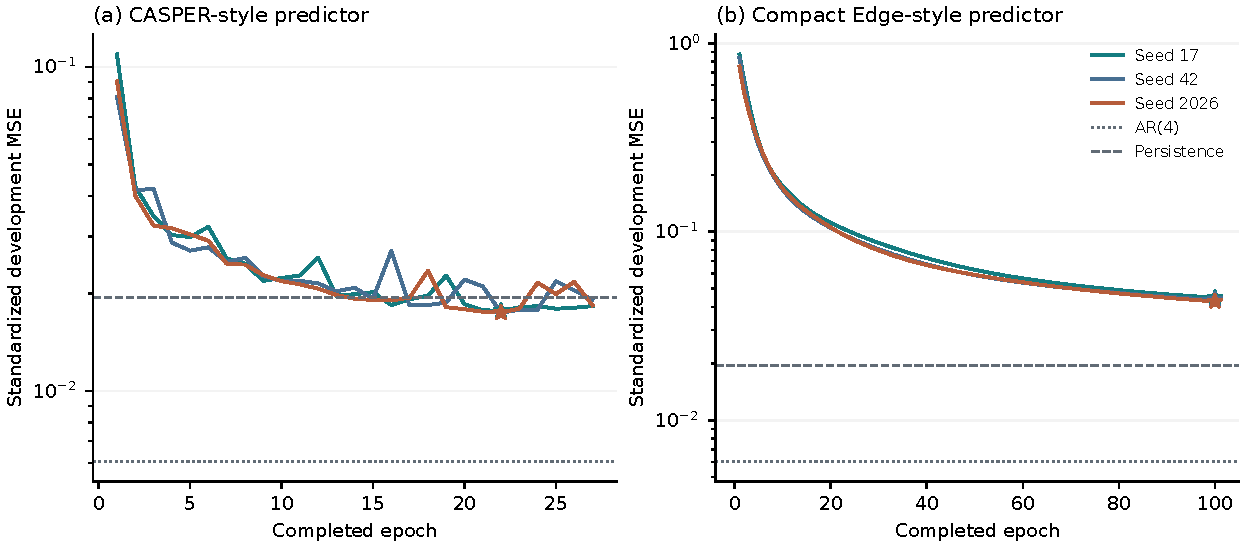
\includegraphics[width=0.85\textwidth]{figures/imu_learning_curves.pdf}
\caption{Saved E3 normal-development learning curves for all neural seeds, with controls on the same targets. Patience stopping supports the adequacy of this bounded CASPER-style fit; the compact model remains limited by the epoch ceiling. These curves do not establish full-paper reproduction or attack-detection superiority.}\label{fig:imu}
\end{figure*}

Median filtering changes the prediction task and induces dependence. These normal-development errors support retaining ordinary predictors, but cannot establish attack-detection superiority or independent generalization.

\subsection{Detection and false-alarm trade-offs}
Table~\ref{tab:audit} reports the complete frozen audit. RBF dual reduces benign alarm points from 7,156 to 7,012, a 2.0123\% reduction below the required 10\%. Q1 deteriorates from 2,397 to 2,522 points, and pooled pre-return gaps increase from two to three. The primary criterion therefore fails. Base and RBF dual overlap all 108 attacks; fresh hits increase from 101 to 105. This secondary gain cannot reverse the declared failure.

\begin{table*}[t]\centering\setlength{\tabcolsep}{4pt}
\caption{All 17 registered E5 methods on 189 synthetic episodes. Benign uses 89,100 points. Hit/fresh means overlap/fresh-onset events out of 108; early is the registered continuity-based count. Clear is timely clears/detected events with return. AP evaluates continuous entry scores, not retained alarm state.}\label{tab:audit}
\begin{tabular}{lrrrrrrr}\toprule
Method & F1 & AP & Benign & Hit/fresh & Early & Gaps & Clear \\\midrule
base point & 0.7809 & 0.7276 & 853 & 108/108 & 14 & 38 & 108/108 \\
base return & 0.6452 & 0.7276 & 6,811 & 108/101 & 1 & 2 & 108/108 \\
base long & 0.6381 & 0.7276 & 7,156 & 108/101 & 1 & 2 & 108/108 \\
base dual & 0.6381 & 0.7276 & 7,156 & 108/101 & 1 & 2 & 108/108 \\
linear point & 0.7799 & 0.7276 & 895 & 108/108 & 14 & 38 & 108/108 \\
linear dual & 0.6336 & 0.7276 & 7,498 & 108/101 & 1 & 2 & 108/108 \\
RBF point & 0.7816 & 0.7276 & 835 & 108/108 & 14 & 39 & 108/108 \\
RBF return & 0.6482 & 0.7276 & 6,652 & 108/105 & 1 & 3 & 108/108 \\
RBF long & 0.6407 & 0.7276 & 7,012 & 108/105 & 1 & 3 & 108/108 \\
RBF dual & 0.6407 & 0.7276 & 7,012 & 108/105 & 1 & 3 & 108/108 \\
RBF dual, no dwell & 0.7644 & 0.7276 & 1,195 & 108/108 & 1 & 1 & 108/108 \\
following point & 0.9202 & 0.9501 & 867 & 108/108 & 108 & 6,692 & 108/108 \\
following dual & 0.7070 & 0.9501 & 7,635 & 108/105 & 90 & 2,970 & 108/108 \\
RBF following dual & 0.7069 & 0.9501 & 7,678 & 108/105 & 90 & 2,979 & 108/108 \\
persistence & 0.0333 & 0.1016 & 527 & 67/67 & 67 & 15,742 & 67/67 \\
mean (21) & 0.0082 & 0.0867 & 84 & 48/48 & 48 & 11,545 & 48/48 \\
base CUSUM & 0.4198 & 0.1967 & 857 & 108/108 & 0 & 0 & 0/108 \\
\bottomrule\end{tabular}

\end{table*}

Figure~\ref{fig:tradeoff} places schedule F1, benign occupancy and lost pre-return support beside one another. Following point has F1 0.9202 and AP 0.9501, exceeding RBF dual's 0.6407 and 0.7276. Yet it has an early falling edge on every attack, with 6,692 pre-return gap points. Following dual reduces these to 90 events and 2,970 points; base dual has one registered early-clear event and two gap points. CUSUM retains support but has no timely clearance. No single plotted axis establishes overall superiority.

\begin{figure*}[t]\centering
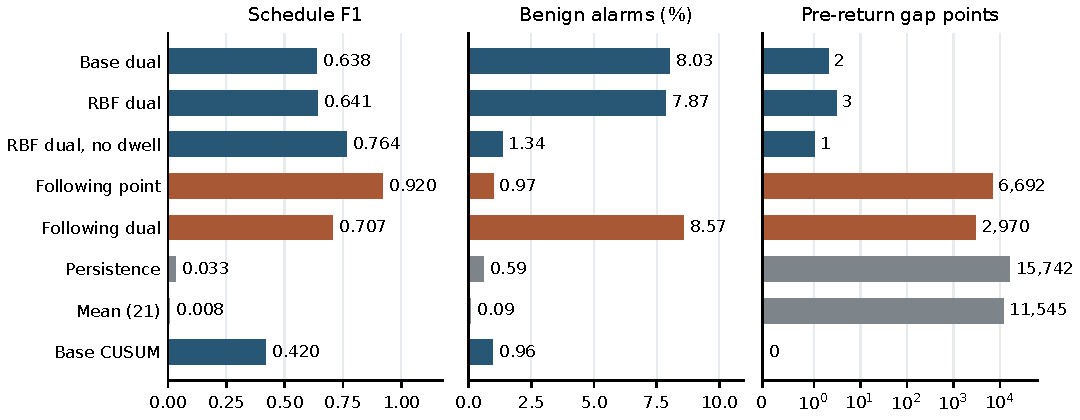
\includegraphics[width=\textwidth]{figures/tradeoffs.pdf}
\caption{Selected contrasts from the complete E5 roster: corruption-schedule F1, benign alarm occupancy and lost alarm support before physical return. Bar labels give saved values; gap axes use a logarithmic scale with a linear region near zero. The figure is a descriptive presentation of the frozen outcomes, not a newly selected primary comparison.}\label{fig:tradeoff}
\end{figure*}

\subsection{Physical return and event interpretation}
Figure~\ref{fig:trace} illustrates the distinction: schedule labels end with command corruption, while displaced motion can continue. Retaining alarm then supports recovery monitoring while reducing schedule precision.

\begin{figure*}[t]\centering
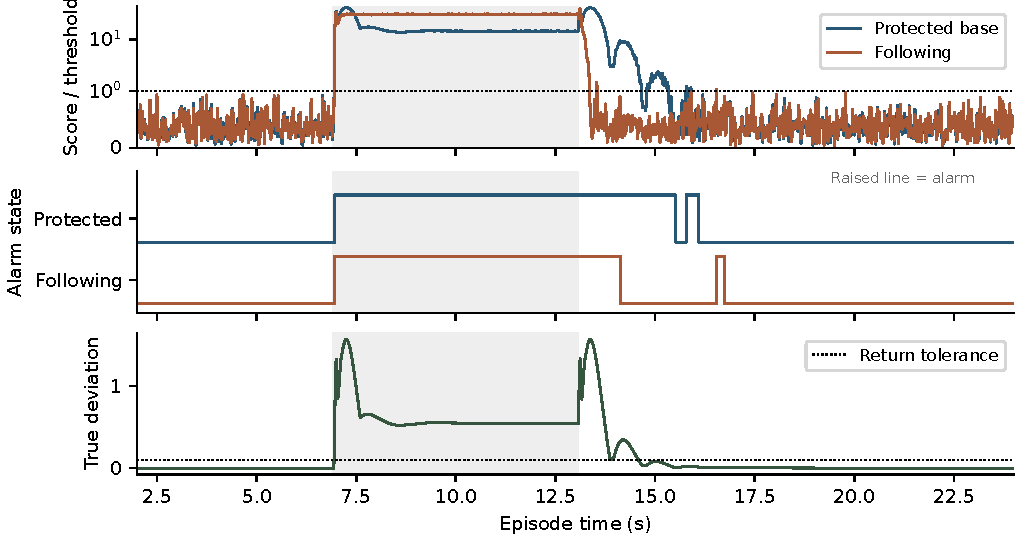
\includegraphics[width=0.81\textwidth]{figures/trace.pdf}
\caption{Post-study illustration from task N14, plant Q2, seed 17, persistent offset. Shading marks command corruption. The following residual falls while physical deviation remains above tolerance. This trace was selected to explain the aggregate contrast; it is not independent confirmatory evidence.}\label{fig:trace}
\end{figure*}

The single RBF early-clear event occurs two samples after onset, with true standardized deviation 0.01649 below tolerance 0.1. A fresh alarm starts three samples later. It is a continuity break, not an outside-tolerance clearance. A separately labelled post-study falling-edge diagnostic finds no outside-tolerance early falls for protected-reference variants, versus 108 events for following point and 82 for following dual. This clarification preserves the registered metric and failed primary decision. Persistence misses 41 events and the rolling mean misses 60; their conditional clearance fractions cannot be presented as recovery success on every event.

\subsection{Ablation and uncertainty studies}
Removing the short window changes zero alarm entries in all 189 episodes. Its contribution is unsupported under these conditions. Removing dwell reduces RBF benign points from 7,012 to 1,195, with 108 overlap hits and 108 timely clears. Its registered early-clear count remains one, on a different episode. Figure~\ref{fig:ablation} separates the component effects. The favorable no-dwell result is an exposed secondary finding; promoting it as a new confirmed detector would require a separately frozen study.

\begin{figure*}[t]\centering
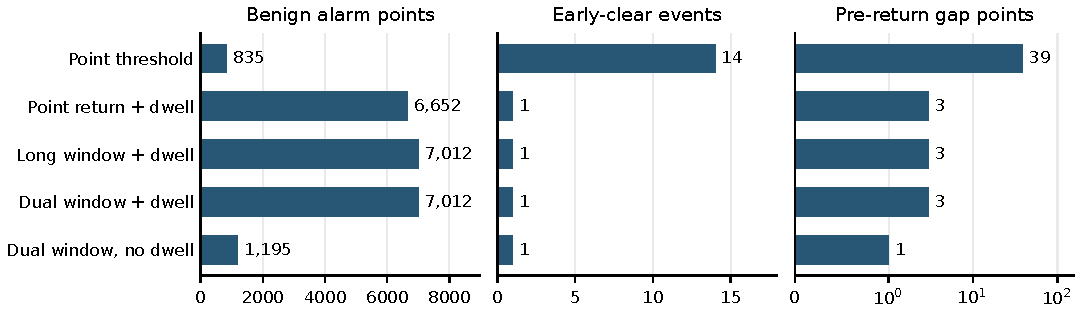
\includegraphics[width=\textwidth]{figures/ablations.pdf}
\caption{Matched RBF alarm-rule variants in E5. Entry score and calibration threshold are shared. The 41-point and dual windows produce identical alarm arrays. Dwell substantially changes benign occupancy; a small gap count alone does not account for missed events or late clearing. All variants detect and timely clear 108 events in this campaign.}\label{fig:ablation}
\end{figure*}

E1 reduces benign points from 621 to 309 using an empirical allowance, but clears only 36/108 detected events with return; its same-entry no-allowance control has 140 benign points and 108 clears. E2 reduces the harder plants' allowances by 51.27\% and 38.56\%, yet fails overall feasibility. Appendix~\ref{app:earlier} retains every earlier comparison under its distinct calibration.

E4 certifies enough normal endpoints on 20/36 constructed traces, failing its all-traces criterion. Averaging competes with temporal correlation and within-window motion. Appendix~\ref{app:uncertainty} gives the complete settings, derivation and outcomes; these are direct synthetic residuals, not attack trials.

\subsection{Computational cost and verification}
E5 normal development takes 16.115 seconds wall and 15.189 seconds worker CPU, with 53.23 MiB sampled peak memory. The final audit takes 27.515 seconds wall and 26.656 seconds CPU, with 90.17 MiB sampled memory and 83.44 MiB outputs. The IMU study takes 764.794 seconds wall, 753.252 seconds CPU and 553.05 MiB sampled memory. These are whole-pipeline measurements with shared work, not isolated inference latency or real-time guarantees.

The final audit passes 25 synthetic software tests and 30,448 saved-artifact checks, including inference replay and separate metric arithmetic. All 3,213 method--episode outcomes remain recorded. These checks support consistency with the declared implementation; they are not independent scientific replication. Appendix~\ref{app:provenance} records budgets, earlier costs and preserved failures.


\section{Discussion}\label{sec:discussion}
\subsection{What the comparisons establish}
The central distinction is between following measured behavior and preserving a reference to approved behavior. Protected evolution retains deviations in this simulator, but the ordinary ARX already provides that benefit. The nonlinear correction and dual-window assembly do not meet the registered improvement target. Existing identification, residual correction, averaging and hysteresis remain close prior art; combining them does not by itself establish an original detector.

Reference accuracy, entry scoring and clearance logic have different roles. The no-dwell contrast shows that persistence can dominate benign occupancy despite unchanged scores and thresholds. AP hides alarm retention; schedule F1 hides much of physical recovery. Both must be accompanied by event and clearance measures.

\subsection{Relationship to published systems}
CASPER and its successor motivate external-sensor prediction; existing hybrid twins and identification methods already establish modeling and correction. E3 does not reproduce their full attack detectors. The Gaussian argument is standard error spending, and the inaccessible full Kaisar et al. architecture leaves an equation-level prior-art comparison unresolved.

MVT-Flow provides a concrete public route to an independent real-robot comparison, but its offline likelihood target differs from online physical-return monitoring. A new comparison must establish compatible features, supervision and output units before claiming that one method improves another. A fault label or a setpoint column alone cannot supply missing attacker semantics or trusted-command provenance.

\subsection{Limitations and next evidence}
Three parameterizations share one simplified simulator. Noise seeds repeat stochastic realizations, not independent plants or acquisitions. Missing physics, trusted initialization and honest sensing limit external validity. The residual diagnostic receives known noise/bias/motion bounds; no operational procedure for estimating all of them is validated. Normal-only IMU development and metadata-only public-data admission do not provide a real-robot recovery test.

voraus-AD supports a separate offline track after features and partitions are frozen. FactoryNet requires source-overlap and release checks. Compatible published-method reproduction and a worthwhile distinct mechanism remain open. The exposed outcomes constrain the next design; they cannot also confirm an outcome-informed replacement.

\section{Conclusion}\label{sec:conclusion}

Attack detection and physical recovery require different evidence. A protected command-driven reference retains deviations that a following predictor can absorb, but model error and alarm persistence create substantial false-alarm costs. The tested nonlinear dual-window candidate fails its declared improvement criterion, and its short window changes no decisions. These results support evaluating reference accuracy, detection and clearance together. They do not establish a novel detector or superiority over CASPER; compatible published-method reproduction and independent recordings remain necessary.


\section*{Declarations}
\paragraph{Funding and competing interests.} No funding or competing interests were declared.
\paragraph{Data and code availability.} Versioned code, configurations, results and a reproducibility inventory are retained locally. No public repository release is claimed. Third-party data remain subject to provider terms; Appendix~\ref{app:provenance} records source identifiers and hashes. All supporting material discussed here is incorporated in this article.
\paragraph{AI assistance and author review.} OpenAI Codex assisted with literature searches, code, experiment execution, analysis, writing and editing. The named author must review the scientific claims and approve the manuscript before submission. No completed human-contribution attestation or independent human review is asserted here.
\appendix
\section{Uncertainty and feasibility}\label{app:uncertainty}
\subsection{Conditional geometric bounds}
Let $\|v\|_s=\max_j|v_j|/s_j$, $d_t=\|x_t-x_t^0\|_s$ and $c_t=\|y_t-r_t\|_s$. If $\|x_t^0-r_t\|_s\le b_t$ and $\|n_t\|_s\le\eta_t$, the triangle and reverse triangle inequalities give
\begin{equation}
 \max(0,c_t-b_t-\eta_t)\le d_t\le c_t+b_t+\eta_t.\label{eq:bound}
\end{equation}
Scalar errors aligned in the same direction attain these extremes. For coordinate error boxes with half-widths $b_{t,j},\eta_{t,j}$, return within $\delta$ holds for every admissible pair exactly when
\begin{equation}
 \max_j\frac{|y_{t,j}-r_{t,j}|+b_{t,j}+\eta_{t,j}}{s_j}\le\delta.\label{eq:box}
\end{equation}
Each coordinate can attain the summed magnitude, proving necessity as well as sufficiency. If any $b_{t,j}+\eta_{t,j}>\delta s_j$, the condition is infeasible. E1 instead tests $c_t+b\le\delta$ with a maximum observed normal discrepancy $b$. That maximum combines model error and noise; Gaussian noise is unbounded. The tested rule is therefore an empirical heuristic, not a verified certificate. Dwell cannot repair $b>\delta$.

\subsection{Covariance-aware window evidence}
For dimensionless residuals write $e_{t,j}=v_{t,j}+\beta_{t,j}+\epsilon_{t,j}$, with $|\beta_{t,j}|\le B_j$ and $|v_{t,j}-v_{t-1,j}|\le L_j$. Assume stationary zero-mean Gaussian AR(1) noise with marginal standard deviation $\sigma_j$ and correlation $0\le\rho_j<1$. Its window-mean variance is
\begin{equation}
 V_{m,j}=\frac{\sigma_j^2}{m^2}\left[m+2\sum_{k=1}^{m-1}(m-k)\rho_j^k\right].\label{eq:covariance}
\end{equation}
For $K$ registered windows and $d$ channels, allocate $\alpha_t=6\alpha/(\pi^2t^2)$ on a clock that never restarts at alarms, and define
\begin{align}
 U_{t,j}(m)={}&|\bar e_{t,j}(m)|+B_j+\frac{L_j(m-1)}2\nonumber\\
 &+\sqrt{2V_{m,j}\log(2dK/\alpha_t)}.\label{eq:windowbound}
\end{align}
With probability at least $1-\alpha$, $|v_{t,j}|\le U_{t,j}(m)$ for every channel, complete registered window and prospective time within a trace. Thus coordinatewise return is certified on that event if
\begin{equation}
 \min_{m\in\mathcal M}U_{t,j}(m)\le\delta_j\quad\text{for every }j.\label{eq:certificate}
\end{equation}
To verify the claim, the two-sided Gaussian tail is at most $\alpha_t/(dK)$. A union bound over channels, windows and times uses $\sum_t\alpha_t=\alpha$. Window overlap and cross-channel dependence do not invalidate that bound. Finally, $|v_{t,j}-\bar v_{t,j}(m)|\le L_j(m-1)/2$ and $|\bar\beta|\le B_j$ yield Equation~\ref{eq:windowbound}. Different channels may select different windows because all bounds hold simultaneously.

This is elementary error spending under supplied assumptions, not new confidence-sequence theory. Invalid observations invalidate affected windows without resetting time. Failure to certify leaves return uncertain and does not generate an attack alarm. Unknown covariance, heavy tails or nonstationarity fall outside the guarantee.

\subsection{Residual experiment and complete results}
E4 fixes $d=4$, windows $\{1,41,201\}$, $\alpha=0.05$, tolerance 0.1 and bias bound 0.01. The four $(\sigma,\rho)$ settings are $(0.03,0)$, $(0.06,0)$, $(0.03,0.8)$ and $(0.06,0.95)$, with channel multipliers $(1,0.8,1.1,0.9)$. Bias is $0.01\cos(0.003t+\phi_j)$ for phases $(0,0.4,0.8,1.2)$. Deviation is zero, $0.02\sin(0.004t+\phi_j)$, or $0.02\sin(0.04t+\phi_j)$; its supplied increment bound is $2a|\sin(\omega/2)|$.

Each trace has 1,200 points and stationary initial noise. Seeds 17, 42 and 2026 supply paired innovations across settings, producing 36 constructed traces. Common support is points 201--1,200. Three fixed-window controls and their simultaneous envelope receive identical residuals/bounds; two deliberately misspecified controls set $\rho=0$ for windows 41 and 201. All 216 outcomes remain recorded. The envelope must certify at least 95\% of common points on every trace. The per-trace probability statement is not simultaneous 95\% coverage across the experiment matrix.

\begin{table*}[t]\centering
\caption{E4 simultaneous-envelope certificates on normal synthetic residuals. Ranges span three seeds with 1,000 common points each. Every trace must reach 95\%; the overall criterion fails.}\label{tab:window}
\begin{tabular}{llrr}\toprule
Noise setting & Deviation profile & Certificates (\%) & Passes \\\midrule
Independent, low & Settled & 100.0--100.0 & 3/3 \\
Independent, low & Slow variation & 100.0--100.0 & 3/3 \\
Independent, low & Faster variation & 100.0--100.0 & 3/3 \\
Independent, high & Settled & 100.0--100.0 & 3/3 \\
Independent, high & Slow variation & 100.0--100.0 & 3/3 \\
Independent, high & Faster variation & 17.2--25.6 & 0/3 \\
Correlated, low & Settled & 100.0--100.0 & 3/3 \\
Correlated, low & Slow variation & 85.8--100.0 & 2/3 \\
Correlated, low & Faster variation & 0.0--0.0 & 0/3 \\
Correlated, high & Settled & 0.0--0.0 & 0/3 \\
Correlated, high & Slow variation & 0.0--0.0 & 0/3 \\
Correlated, high & Faster variation & 0.0--0.0 & 0/3 \\
\bottomrule\end{tabular}

\end{table*}
\begin{figure*}[t]\centering
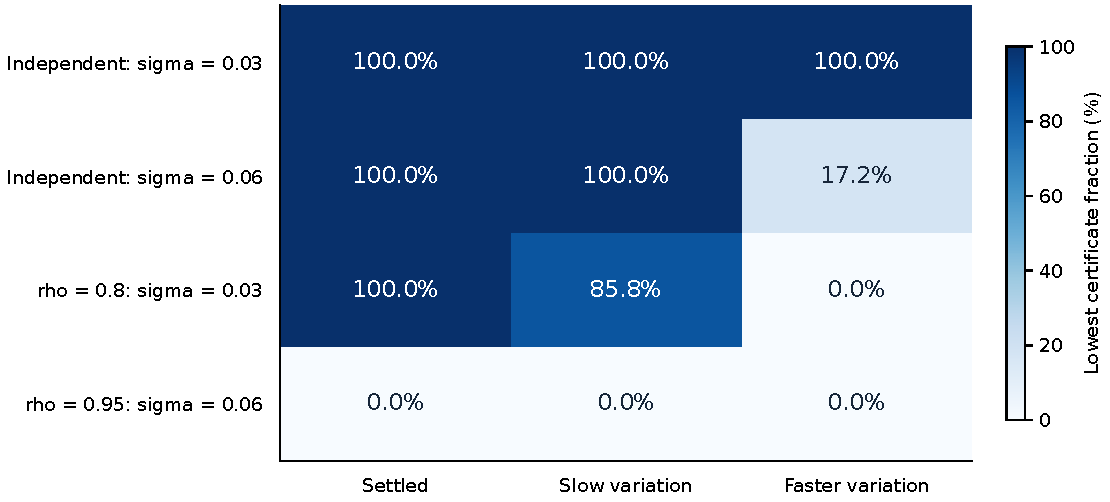
\includegraphics[width=0.62\textwidth]{figures/window_feasibility.pdf}
\caption{Lowest E4 certificate fraction across seeds in each residual condition. All true deviations lie within tolerance. Low certificate coverage means uncertain return under the supplied bounds, not detected attacks.}\label{fig:window}
\end{figure*}

The envelope passes 20/36 traces. Instantaneous evidence certifies none. Under independent low noise with faster variation, window 41 certifies every point while 201 certifies none: the longer drift allowance outweighs averaging. Under correlated low noise with slow variation, fractions are 100\%, 85.8\% and 100\%; their 95.27\% average does not satisfy the all-traces rule. At $(0.06,0.95)$ no valid control certifies even settled motion. The misspecified 201-point control would certify 91.53\% on average there, without a valid covariance guarantee.

This generator constructs residuals directly and supplies the bounds; it does not simulate robot dynamics or attacks. All deviations are within tolerance, so the absence of observed bound violations cannot establish rare unsafe-clearing risk. Operational estimation of the assumptions and behavior near the tolerance boundary remain untested.

\section{Earlier comparisons and full final metrics}\label{app:earlier}

\subsection{E1: original recovery comparison}
E1 comprises 216 episodes and 13 methods, with 237,600 eligible points and 135 intervention events. Twenty-seven events have missing command context. Nineteen clean episodes provide 20,900 eligible calibration points; the principal state-machine threshold search allows at most 209 alarmed points on this finite population. This differs from the final audit's point-quantile calibration. The additional constant episode band uses rank 19 of 19 episode maxima; shifted tasks do not establish exchangeability or conformal coverage. Matched-entry ablations preserve their own realized alarm burdens.
\begin{table*}[t]\centering
\caption{E1 attack and recovery outcomes, retained from the saved presentation. Clearance counts condition on detected events with measured return.}
\setlength{\tabcolsep}{3pt}\begin{tabular}{lrrrrr}\toprule
Method & Benign & F1 & Overlap/fresh & Early & Clear/return \\\midrule
Persistence & 878 & 0.057 & 127/127 & 127 & 127/127 \\
ARX one-step & 792 & 0.803 & 108/108 & 108 & 108/108 \\
Following point & 794 & 0.808 & 108/108 & 108 & 108/108 \\
Following hysteresis & 993 & 0.785 & 108/108 & 108 & 108/108 \\
Nominal hysteresis & 789 & 0.713 & 108/108 & 45 & 108/108 \\
Nominal fixed return & 621 & 0.657 & 108/108 & 0 & 108/108 \\
Learned point & 819 & 0.700 & 108/108 & 18 & 108/108 \\
Learned hysteresis & 792 & 0.683 & 108/108 & 0 & 108/108 \\
Learned fixed return & 827 & 0.690 & 108/108 & 0 & 108/108 \\
Uncertainty return & 309 & 0.446 & 108/104 & 0 & 36/108 \\
Episode CP band & 0 & 0.744 & 108/108 & 75 & 108/108 \\
Matched no allowance & 140 & 0.709 & 108/108 & 0 & 108/108 \\
Matched no dwell & 20 & 0.453 & 108/108 & 0 & 36/108 \\
\bottomrule\end{tabular}

\end{table*}
\begin{table*}[t]\centering
\caption{E1 additional metrics. Unknown states remain eligible, cannot count as detections, and receive AP score $-1$, below valid nonnegative scores.}
\setlength{\tabcolsep}{3pt}\begin{tabular}{lrrrrrr}\toprule
Method & Precision & Recall & AP & Episodes/h & Missed & Known (\%) \\\midrule
Persistence & 0.203 & 0.033 & 0.130 & 480.8 & 8 & 100.0 \\
ARX one-step & 0.868 & 0.748 & 0.770 & 1426.3 & 27 & 90.0 \\
Following point & 0.878 & 0.747 & 0.770 & 793.9 & 27 & 90.0 \\
Following hysteresis & 0.841 & 0.735 & 0.770 & 99.0 & 27 & 90.0 \\
Nominal hysteresis & 0.706 & 0.719 & 0.587 & 84.8 & 27 & 90.0 \\
Nominal fixed return & 0.656 & 0.658 & 0.587 & 48.5 & 27 & 90.0 \\
Learned point & 0.658 & 0.748 & 0.589 & 1054.5 & 27 & 90.0 \\
Learned hysteresis & 0.628 & 0.747 & 0.589 & 62.6 & 27 & 90.0 \\
Learned fixed return & 0.641 & 0.747 & 0.589 & 115.2 & 27 & 90.0 \\
Uncertainty return & 0.318 & 0.747 & 0.589 & 26.3 & 27 & 90.0 \\
Episode CP band & 0.742 & 0.746 & 0.589 & 0.0 & 27 & 90.0 \\
Matched no allowance & 0.675 & 0.747 & 0.589 & 28.3 & 27 & 90.0 \\
Matched no dwell & 0.325 & 0.747 & 0.589 & 28.3 & 27 & 90.0 \\
\bottomrule\end{tabular}

\end{table*}
\subsection{E2: normal commissioning}
The finite grid contains ARX orders 4, 8, 16 and 32 and finite impulse response lengths 16, 32 and 64, each with ridge $10^{-7}$, $10^{-5}$ or $10^{-3}$, on three plants: 63 fits. Fitting and selection precede 81 new normal episodes. The selected orders are 8, 16 and 32 with ridge $10^{-7}$. Table~\ref{tab:normalall} retains distinct prediction roles. Forced-latch probes measure normal clearance feasibility, not post-attack recovery. The hard-plant reductions in empirical allowance do not establish a probabilistic or deterministic error bound.
\begin{table*}[t]\centering
\caption{E2 complete normal-reference comparison. Each row has 29,700 eligible observations and 108 forced-latch probes. Selected reference and selected ARX are identical and appear once.}\label{tab:normalall}
\setlength{\tabcolsep}{4pt}\begin{tabular}{llrrrr}\toprule
Plant & Reference & RMSE & Allowance & Feasible (\%) & Clear/probes \\\midrule
Q1 & ARX(4), free & 0.00948 & 0.0553 & 99.80 & 108/108 \\
Q1 & Selected ARX, free & 0.00934 & 0.0553 & 99.82 & 108/108 \\
Q1 & Selected FIR & 0.01211 & 0.2322 & 0.00 & 0/108 \\
Q1 & ARX(4), one-step & 0.00976 & 0.0649 & 97.92 & 108/108 \\
Q1 & Command as state & 0.09584 & 2.1344 & 0.00 & 0/108 \\
Q2 & ARX(4), free & 0.01020 & 0.1469 & 0.00 & 0/108 \\
Q2 & Selected ARX, free & 0.00972 & 0.0716 & 93.32 & 108/108 \\
Q2 & Selected FIR & 0.01693 & 0.3971 & 0.00 & 0/108 \\
Q2 & ARX(4), one-step & 0.01036 & 0.1211 & 0.00 & 0/108 \\
Q2 & Command as state & 0.10423 & 2.1528 & 0.00 & 0/108 \\
Q3 & ARX(4), free & 0.01586 & 0.1913 & 0.00 & 0/108 \\
Q3 & Selected ARX, free & 0.01439 & 0.1175 & 0.00 & 0/108 \\
Q3 & Selected FIR & 0.02215 & 0.4596 & 0.00 & 0/108 \\
Q3 & ARX(4), one-step & 0.01573 & 0.1807 & 0.00 & 0/108 \\
Q3 & Command as state & 0.11251 & 2.2058 & 0.00 & 0/108 \\
\bottomrule\end{tabular}

\end{table*}
\subsection{E5: complete additional metrics and plant strata}
The following tables complement the complete 17-method audit in Table~\ref{tab:audit}. Alarm starts per hour use the total eligible duration of wholly benign episodes. Their high frequency for point rules reflects repeated short excursions; the metric should be read alongside occupancy. No unknown-state denominator trimming is applied to this audit. All 189 episodes and 3,213 outcomes are retained.
\begin{table*}[t]\centering
\caption{Final audit: unadjusted point precision/recall, benign occupancy, alarm starts per benign hour and missed events.}
\begin{tabular}{lrrrrr}\toprule
Method & Precision & Recall & Benign (\%) & Starts/h & Misses \\\midrule
base point & 0.6434 & 0.9931 & 0.957 & 1537.4 & 0 \\
base return & 0.4777 & 0.9936 & 7.644 & 1208.1 & 0 \\
base long & 0.4699 & 0.9936 & 8.031 & 1208.1 & 0 \\
base dual & 0.4699 & 0.9936 & 8.031 & 1208.1 & 0 \\
linear point & 0.6421 & 0.9930 & 1.004 & 1618.2 & 0 \\
linear dual & 0.4651 & 0.9934 & 8.415 & 1270.7 & 0 \\
RBF point & 0.6445 & 0.9929 & 0.937 & 1501.0 & 0 \\
RBF return & 0.4811 & 0.9932 & 7.466 & 1191.9 & 0 \\
RBF long & 0.4729 & 0.9932 & 7.870 & 1191.9 & 0 \\
RBF dual & 0.4729 & 0.9932 & 7.870 & 1191.9 & 0 \\
RBF dual, no dwell & 0.6214 & 0.9929 & 1.341 & 1501.0 & 0 \\
following point & 0.8575 & 0.9930 & 0.973 & 1618.2 & 0 \\
following dual & 0.5487 & 0.9934 & 8.569 & 1331.3 & 0 \\
RBF following dual & 0.5486 & 0.9934 & 8.617 & 1317.2 & 0 \\
persistence & 0.1286 & 0.0192 & 0.591 & 274.7 & 41 \\
mean (21) & 0.0385 & 0.0046 & 0.094 & 78.8 & 60 \\
base CUSUM & 0.2665 & 0.9887 & 0.962 & 301.0 & 0 \\
\bottomrule\end{tabular}

\end{table*}
\begin{table*}[t]\centering
\caption{Primary base-dual versus RBF-dual comparison by plant. Every plant has 29,700 benign points and 36 attack events.}
\setlength{\tabcolsep}{4pt}\begin{tabular}{lrrrrrr}\toprule
Plant & Base benign & RBF benign & Base gaps & RBF gaps & Base fresh & RBF fresh \\\midrule
Q1 & 2397 & 2522 & 0 & 0 & 36 & 36 \\
Q2 & 2646 & 2532 & 2 & 3 & 29 & 33 \\
Q3 & 2113 & 1958 & 0 & 0 & 36 & 36 \\
\bottomrule\end{tabular}

\end{table*}

\section{Reproducibility and source identities}\label{app:provenance}
\subsection{Recorded execution and failures}
Versioned records retain inputs, configurations, commands, dependencies, code revisions, logs and every outcome. E1--E5 correspond respectively to \path{recovery_v0.8}, \path{commissioning_v0.9}, \path{casper_convergence_v0.11}, \path{return_bound_v0.12}, and \path{residual_twin_v0.13} followed by \path{attack_audit_v0.14}. Their calibration policies are not interchangeable. No experiment was rerun for this article revision.

E1 consumed 229.20 s wall, 228.07 s CPU and 167.25 MiB sampled memory; E2 consumed 14.75 s, 14.30 s and 113.97 MiB. E1's initial launch failed before initialization because monitoring was blocked. E2 stopped once on a reporting-key collision after selection; the recorded repair preserved identical fits before fresh generation. E5 has no failed scientific attempt. Its final limits were 120 s wall, 90 s CPU, 1 GiB monitored memory and 128 MiB output. Worker peak memory was 99.53 MiB versus 90.17 MiB sampled; sampling is not an instantaneous hard bound. The IMU run used 2.68 MiB outputs and passed 17 synthetic tests and 3,754 saved-artifact checks. E4 used 0.565 s wall, 0.459 s CPU, 39.81 MiB memory and 11.07 MiB outputs, with 20 tests and 2,665 checks.

The final freeze SHA-256 is \path{b48a0c3927b465559a8f7b372c2d26ed7148642c97d2435de83995a0ad3be021}; its result-package manifest is \path{987d8904dda988c7ccd51d61a5e52cf8e162e8f0156286aad89c385813b785dc}. Asset receipts bind figures and tables to saved results. Identifiers establish provenance, not validity. Raw data and third-party manuscripts are excluded from the editable archive.

\subsection{Real-data identity and comparator admission}
The author-linked CASPER-1-and-2 provider-v2 nominal IMU file has SHA-256 \path{1221df9be80c229969f3f21f820837e68ad28f4ccb3949bf4013f00d6d69d62c}. Its original-paper run and clock correspondence remain unresolved.

The original voraus-AD file is linked by \url{https://github.com/vorausrobotik/voraus-ad-dataset}. It has 1,115,942,833 bytes and SHA-256 \path{c90ab1c78af52651b954d41787f7e89d750f0a128b57600b0e5ceec22621f704}. Data are CC BY-NC-SA 4.0; code is MIT. Metadata verify 2,321,690 rows, 137 columns and the 2,122 executions in Table~\ref{tab:data}. Setting 72 (PRE\_A) supplies all 948 training executions. Within-execution time resets to zero, increases strictly with increments 0.00845194--0.01211095 s, and does not establish absolute acquisition order. Maximum train/test lengths are both 1,164 rows. Process signals remain unopened.

Pinned MVT-Flow code \path{a91a86a642d23df58833b792a53de01edfd81abe} has four coupling blocks, clamp 1.2, width scale two, Adam $8\times10^{-4}$, batch 32 and 70 epochs. It computes test AUROC each epoch but saves the fixed final epoch; this alone does not prove test-based selection. Training uses $\|z\|^2-\log|J|$, while paper/scoring use $\tfrac12\|z\|^2-\log|J|$. The paper describes three convolutions; the default released block constructs two. A padding truncation is overwritten, but the received release has no overlength test execution, so no impact is demonstrated. These findings leave faithful reproduction unresolved; they do not prove invalid published results.

FactoryNet arXiv:2605.09081v5 (8 October 2026) reports ICML-associated workshop acceptance, not verified main-conference publication. The pinned data card \path{3bea3cfc10545d898604f93170108576fd46d518} reports 56,591 executions: 14,847 real and 41,744 simulated. Code revision is \path{651f066d97b704f0824687f1086eeb8f0422a8f3}. The card says Isaac Sim 5.1 data are still uploading; the available snapshot is 4.5. Imported voraus-AD, AURSAD and CNC are not independent new acquisitions. Context includes fault labels, channels vary by embodiment, and licenses differ by subset/code. No observations were downloaded or performance measured.

\begingroup\raggedright
\begin{thebibliography}{20}

\bibitem{securitysurvey} Abdul Rehman Qureshi, Adrián Asensio, Muhammad Imran, Jordi Garcia, Xavi Masip-Bruin. {A survey on security enhancing Digital Twins: Models, applications and tools}. \emph{Computer Communications, 238:108158}, 2025. Article 108158. \url{https://doi.org/10.1016/j.comcom.2025.108158}.

\bibitem{lifecycle} Taru Itäpelto, Mohammed Elhajj, Marten van Sinderen. {Digital twin application in lifecycle security of critical infrastructures: A systematic literature review}. \emph{International Journal of Critical Infrastructure Protection, 50:100783}, 2025. Article 100783. \url{https://doi.org/10.1016/j.ijcip.2025.100783}.

\bibitem{casper} Hakan Kayan, Ryan Heartfield, Omer Rana, Pete Burnap, Charith Perera. {CASPER: Context-Aware IoT Anomaly Detection System for Industrial Robotic Arms}. \emph{ACM Transactions on Internet of Things, 5(3):1--36}, 2024. Article 18. \url{https://doi.org/10.1145/3670414}.

\bibitem{edge} Hakan Kayan, Ryan Heartfield, Omer Rana, Pete Burnap, Charith Perera. {Real-Time Anomaly Detection for Industrial Robotic Arms Using Edge Computing}. \emph{IEEE Internet of Things Journal, 12(15):29696--29712}, 2025. \url{https://doi.org/10.1109/JIOT.2025.3569780}.

\bibitem{hybrid} Samuel Ayankoso, Eric Kaigom, Hassna Louadah, Hamidreza Faham, Fengshou Gu, Andrew Ball. {A Hybrid Digital Twin Scheme for the Condition Monitoring of Industrial Collaborative Robots}. \emph{Procedia Computer Science, 232:1099--1108}, 2024. \url{https://doi.org/10.1016/j.procs.2024.01.108}.

\bibitem{arp} Daniel Arp, Erwin Quiring, Feargus Pendlebury, et al. {Pitfalls in Machine Learning for Computer Security}. \emph{Communications of the ACM, 67(11):104--112}, 2024. \url{https://doi.org/10.1145/3643456}.

\bibitem{calibration} Tinghui Chen, Weiyi Yang, Shuai Li, Xin Luo. {Data-Driven Calibration of Industrial Robots: A Comprehensive Survey}. \emph{IEEE/CAA Journal of Automatica Sinica, 12(8):1544--1567}, 2025. \url{https://doi.org/10.1109/jas.2025.125237}.

\bibitem{identification} Koen Classens, Rodrigo A. Gonz{\'a}lez, Tom Oomen. {Recursive identification of structured systems: An instrumental-variable approach applied to mechanical systems}. \emph{European Journal of Control, 84:101238}, 2025. \url{https://doi.org/10.1016/j.ejcon.2025.101238}.

\bibitem{voraus} Jan Thieß Brockmann, Marco Rudolph, Bodo Rosenhahn, Bastian Wandt. {The voraus-AD Dataset for Anomaly Detection in Robot Applications}. \emph{IEEE Transactions on Robotics, 40:438--451}, 2024. \url{https://doi.org/10.1109/tro.2023.3332224}.

\bibitem{factory} Jonas Petersen, Pratik Jawahar, Riccardo Maggioni, et al. {FactoryNet: A Large-Scale Dataset toward Industrial Time-Series Foundation Models}. \emph{arXiv preprint}, 2026. Preprint, version 5, 8 October 2026; arXiv:2605.09081. \url{https://arxiv.org/abs/2605.09081v5}.

\bibitem{moderntcn} Donghao Luo, Xue Wang. {ModernTCN: A Modern Pure Convolution Structure for General Time Series Analysis}. \emph{International Conference on Learning Representations}, 2024. \url{https://openreview.net/forum?id=vpJMJerXHU}.

\bibitem{itransformer} Yong Liu, Tengge Hu, Haoran Zhang, et al. {iTransformer: Inverted Transformers Are Effective for Time Series Forecasting}. \emph{International Conference on Learning Representations}, 2024. \url{https://openreview.net/forum?id=JePfAI8fah}.

\newpage

\bibitem{timemixer} Shiyu Wang, Haixu Wu, Xiaoming Shi, et al. {TimeMixer: Decomposable Multiscale Mixing for Time Series Forecasting}. \emph{International Conference on Learning Representations}, 2024. \url{https://openreview.net/forum?id=7oLshfEIC2}.

\bibitem{interval} Jordi Meseguer, Vicen{\c c} Puig, Teresa Escobet, Jordi Saludes. {Observer gain effect in linear interval observer-based fault detection}. \emph{Journal of Process Control, 20(8):944--956}, 2010. \url{https://doi.org/10.1016/j.jprocont.2010.06.017}.

\bibitem{fail} Chen Xu, Tony Khuong Nguyen, Emma Dixon, et al. {Can We Detect Failures Without Failure Data? Uncertainty-Aware Runtime Failure Detection for Imitation Learning Policies}. \emph{Robotics: Science and Systems XXI}, 2025. \url{https://doi.org/10.15607/RSS.2025.XXI.073}.

\bibitem{howard} Steven R. Howard, Aaditya Ramdas, Jon McAuliffe, Jasjeet Sekhon. {Time-uniform, nonparametric, nonasymptotic confidence sequences}. \emph{The Annals of Statistics, 49(2):1055--1080}, 2021. \url{https://doi.org/10.1214/20-AOS1991}.

\bibitem{kaisar} H. Kaisar, M. Rehan, I. Ahmed, M. Bilal, M. Khalid. {A Digital Twin-Based Cybersecurity Architecture for FDI Anomaly Detection and Isolation in Next Generation Robotic Vehicles}. \emph{IEEE Open Journal of the Communications Society, 7:12709--12728}, 2026. \url{https://doi.org/10.1109/OJCOMS.2026.3739185}.

\bibitem{rescue} David Ahmedt-Aristizabal, Abdelwahed Khamis, Mohammad Ali Armin, Lars Petersson. {RESCUE: Is This Alarm Worth Acting On? Counterfactual Evaluation of VLA Runtime Monitors}. \emph{arXiv preprint}, 2026. Preprint, version 1, 9 October 2026; arXiv:2610.13516. \url{https://arxiv.org/abs/2610.13516v1}.

\bibitem{tsbad} Qinghua Liu, John Paparrizos. {The Elephant in the Room: Towards A Reliable Time-Series Anomaly Detection Benchmark}. \emph{Advances in Neural Information Processing Systems 37, 108231--108261}, 2024. \url{https://doi.org/10.52202/079017-3437}.

\bibitem{vus} Paul Boniol, Ashwin K. Krishna, Marine Bruel, et al. {VUS: effective and efficient accuracy measures for time-series anomaly detection}. \emph{The VLDB Journal, 34(3)}, 2025. Article 32. \url{https://doi.org/10.1007/s00778-025-00907-x}.

\end{thebibliography}

\endgroup
\end{document}
